\subsection{蒸发法}
蒸发法生长晶体的基本原理是将溶剂不断蒸发移去,而使溶液保持在过饱和状态,从而使晶体不断生长,这种方法比较适合于溶解度较大而其温度系数很小或是具有负温度系数的物质(表3.8)。蒸发法和流动法一样,晶体生长也是在恒温下进行的。不同是流动法用补充溶质,而蒸发法用移去溶剂来造成过饱和度。

蒸发法生长晶体的装置和降温法的装置十分类似。所不同的是在降温法中,育晶器中蒸发产生的冷凝水全部回流,而蒸发法则是部分回流。降温法通过降温速度来控制过饱和度,而蒸发法则是通过控制回流比(蒸发量)来控制过饱和度的。

\begin{table}[h]
\centering
\caption{一些适用于蒸发法生长的晶体在60℃时的溶解度及其温度系数}
\begin{tabular}{c|c|c}\toprule
物质 & \tabincell{c}{溶解度\\(g/1000g溶液)} & \tabincell{c}{溶解度温度系数\\g/1000g溶液$\cdot$℃}\\\hline
$\rm K_4HPO_4$ & 720 & $+0.1$\\
$\rm Li_2SO_4\cdot H_2O$ & 244 & $-0.36$\\
$\rm LiIO_3$ & 431 & $0.2$\\
\bottomrule
\end{tabular}
\end{table}

蒸发法生长晶体的装置有许多类型。图3.23示出的是比较简单的一种:在严格密封的育晶器上方设置冷凝器(可通水冷却)。溶剂自溶液表面不断蒸发,水蒸汽在冷凝器上凝结,并积聚在其下方的小杯内,再用虹吸管按控制量移出育晶器外,在晶体生长过程中,取水速度应小于冷凝速度,使大部分冷凝水(包括器壁上的)回流到液面上去,否则液面上易产生自发结晶。这种装置比较适合在较高的生长温度($>$60℃)使用。温度较低。蒸发量太小,不能满足晶体生长的需要。

\begin{figure}[htb]
 \centering
 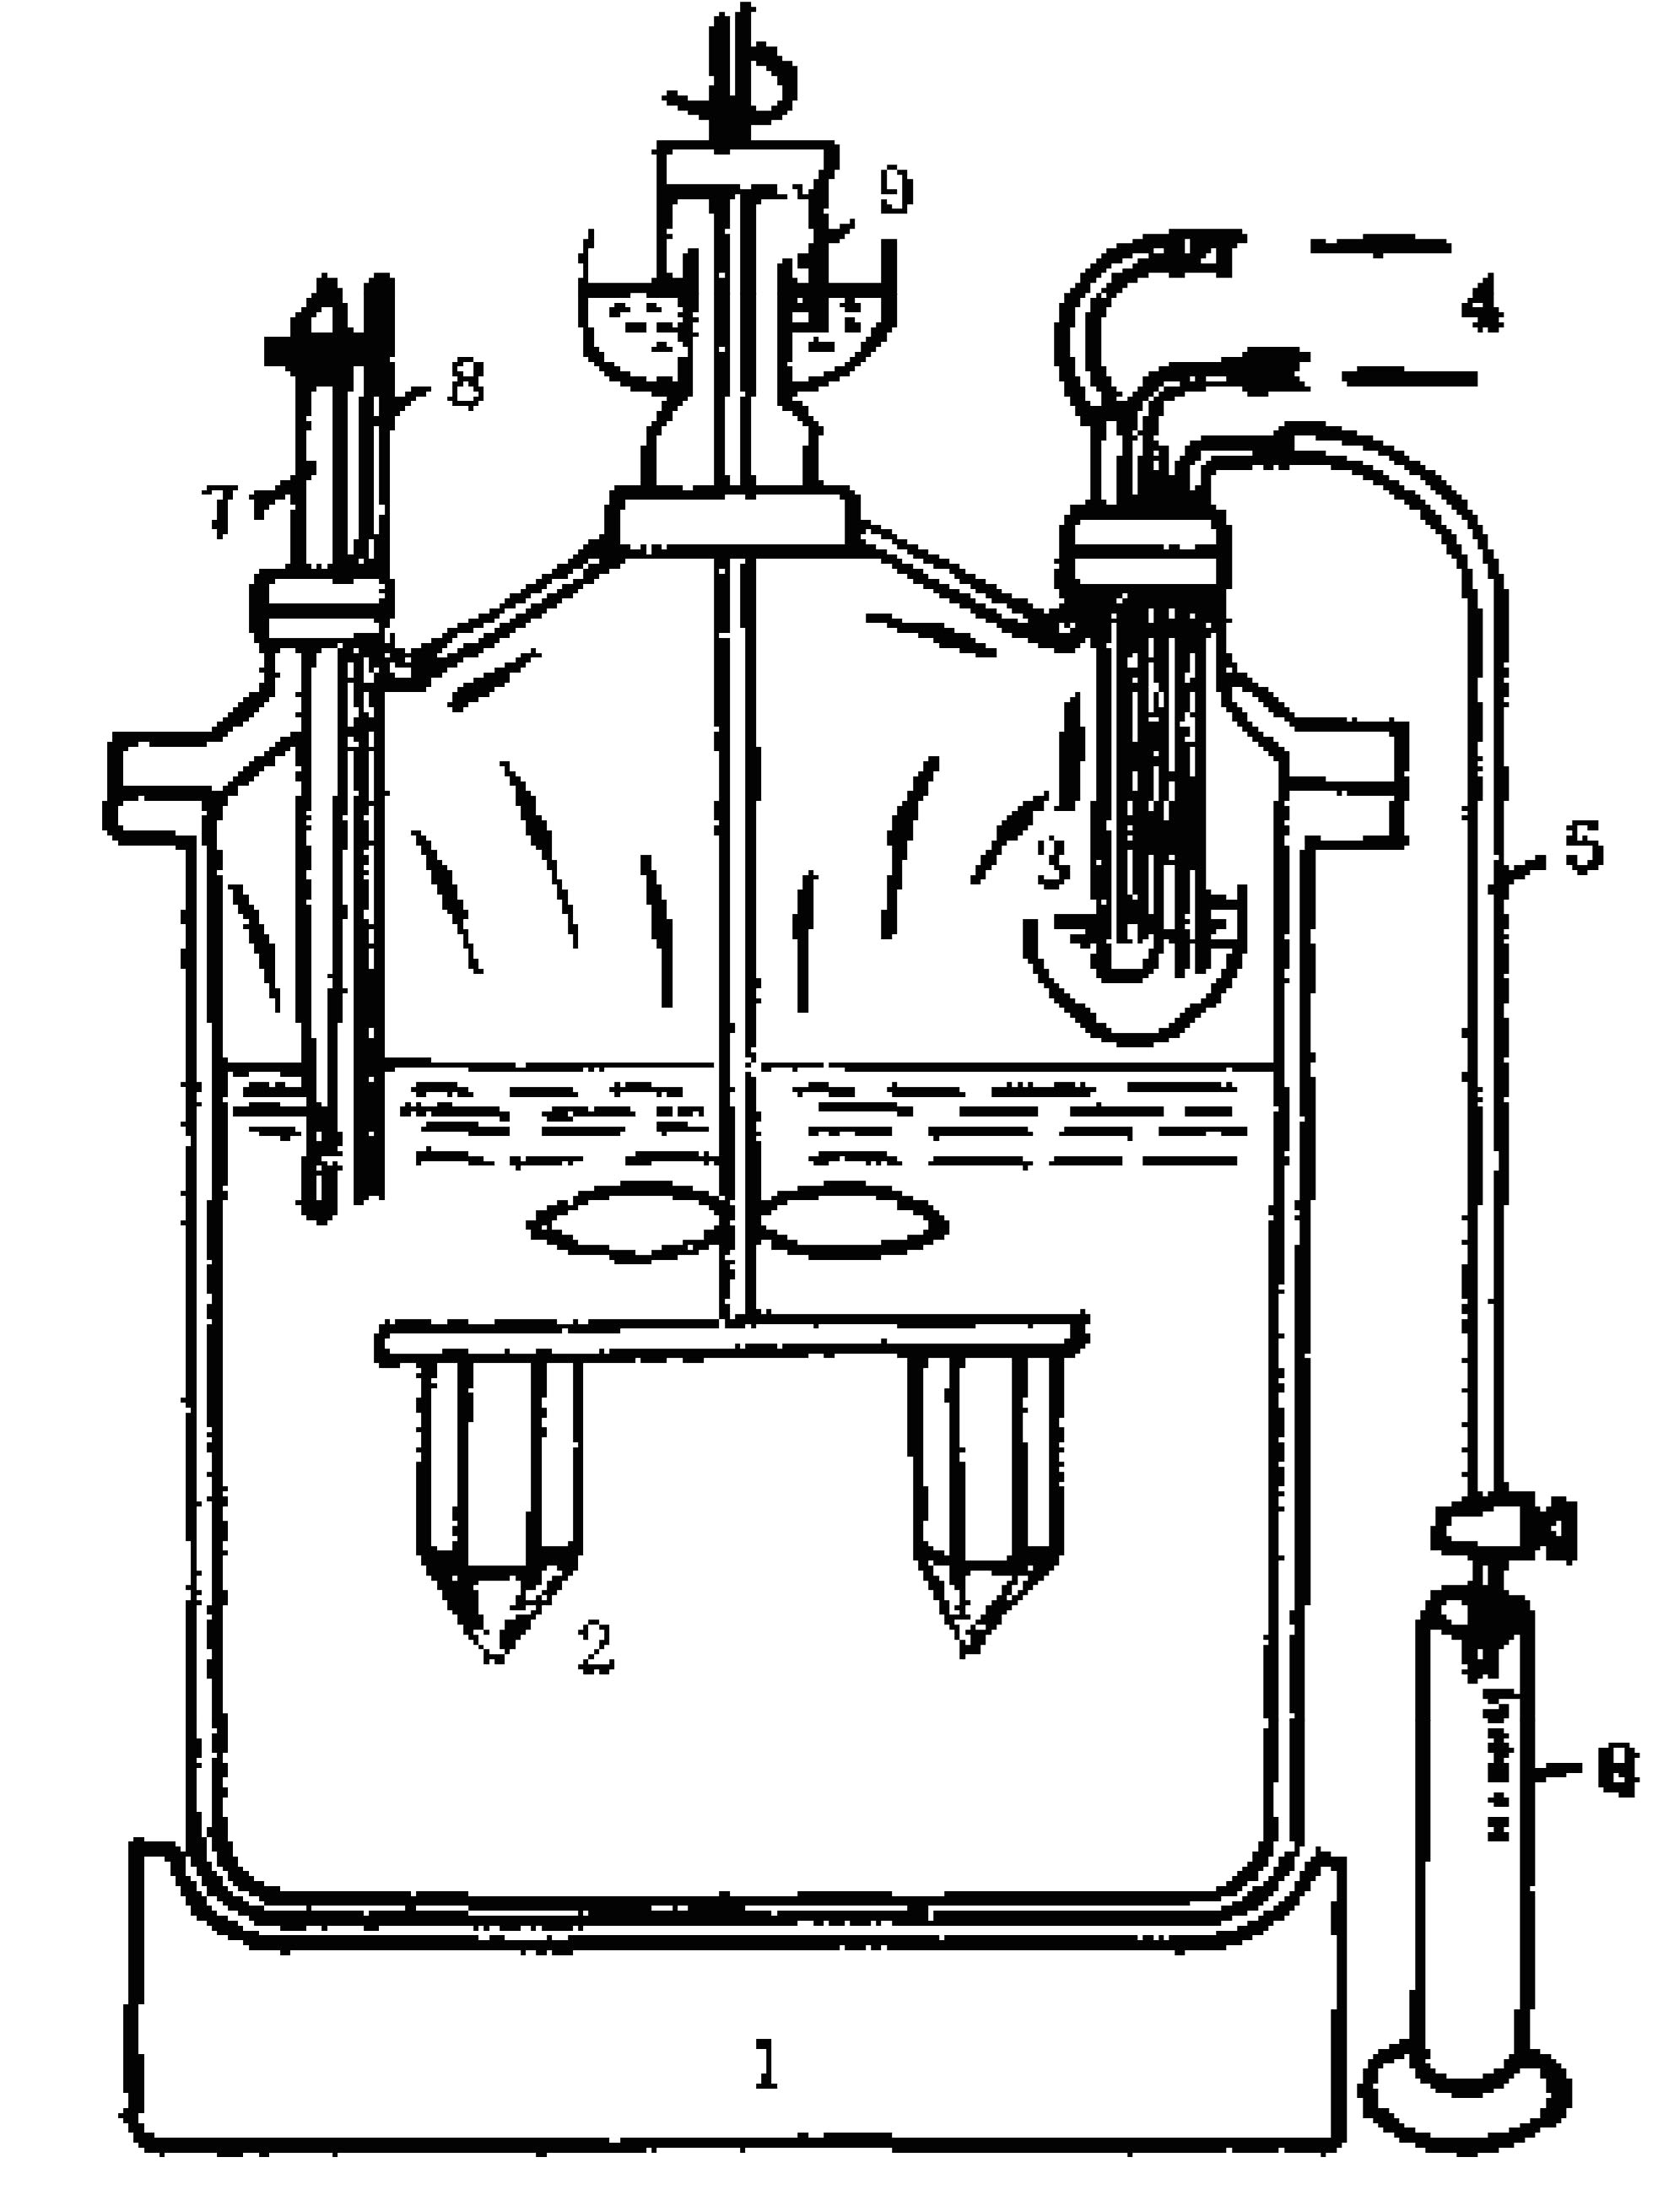
\includegraphics[width=0.4\textwidth]{fig/cp03/img3.23.jpg}
 \caption{蒸发法育晶装置。}
\end{figure}

\begin{figure}[hbt]
 \centering
 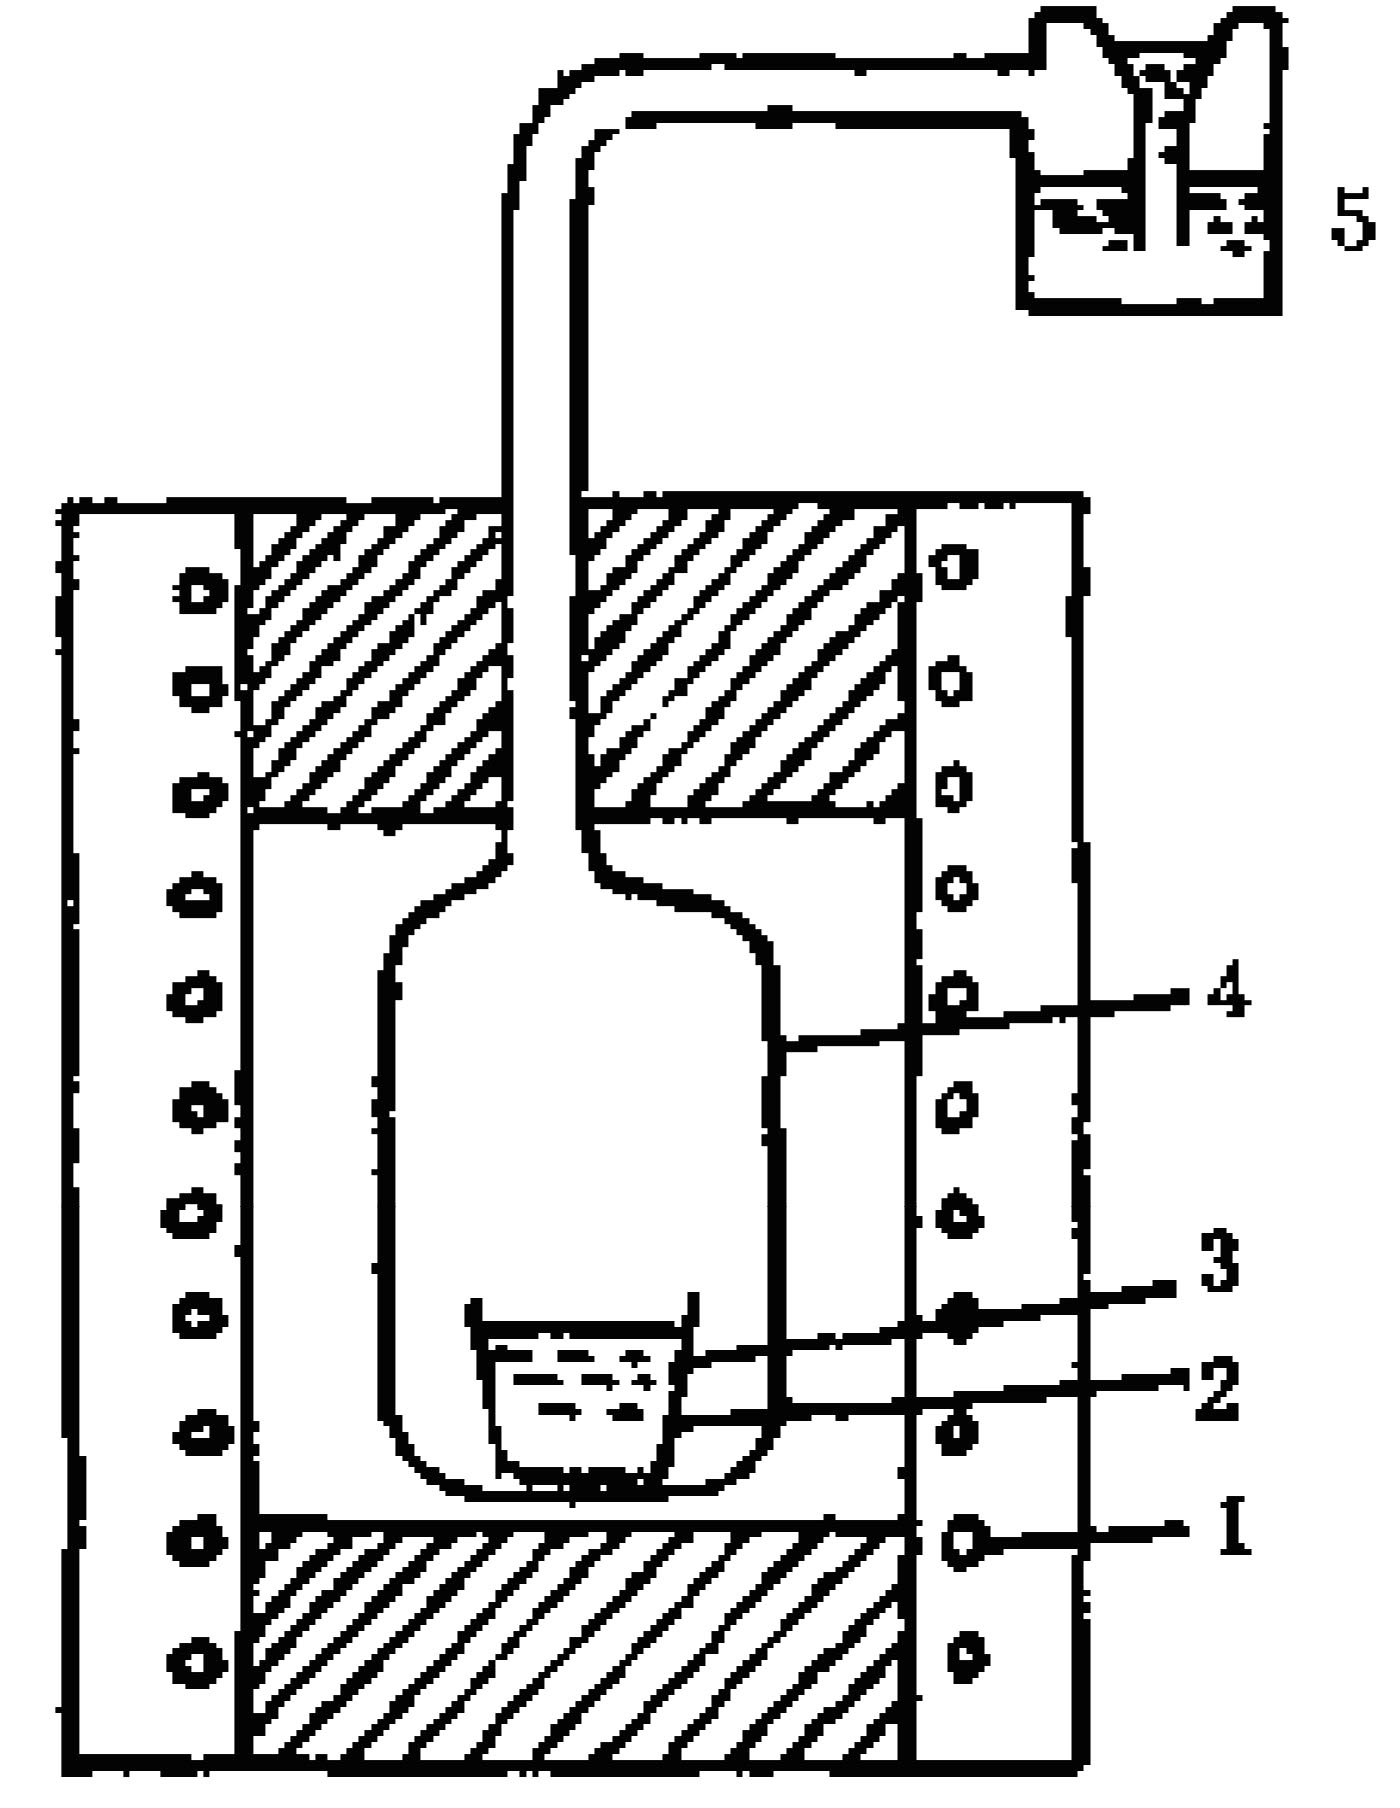
\includegraphics[width=0.4\textwidth]{fig/cp03/img3.24.jpg}
 \caption{生长NdPP晶体的装置。}
\end{figure}

有时体系中某一成分(如水)的蒸发并不是作为溶剂蒸发直接导致晶体生长,而是引起化学反应,间接导致晶体生长,例如在$\rm Nd_2O_3-H_3PO_4$(或$\rm Nd_2O_3-P_2O_5-H_2O$)体系中生长五磷酸钕($\rm NdP_5O_{14}$简称NdPP)晶体,其形成机制可能是
$$ \rm 14\ H_3PO_4 + Nd_2O_3 \xrightarrow{>260℃} 2\ NdP_5O_{14}+2\ H_4P_2O_7+17\ H_2O\uparrow$$

NdPP在焦磷酸($\rm H_4P_2O_7$)中有较大的溶解度,所以不会从溶液中析出,当温度升至300℃以上,焦磷酸逐渐脱水,形成多聚偏磷酸,NdPP在其中溶解度很小,在升温和蒸发过程中,由于焦磷酸浓度降低而使NdPP在溶液中到达过饱和而结晶出来
$$\rm n\ H_4P_2O_7 + NdP_5O_{14} \xrightarrow{>300℃} 2\ (HPO_3)_n + NdP_5O_{14}\downarrow + n\ H_2O\uparrow $$

据此机理,采用图3.24所示装置,在一定的温度下,控制水的蒸发速率就可以生长出质量较好的NdPP晶体。

这种晶体生长方式实际上是晶体在无机溶剂(焦磷酸)的溶液中,通过焦磷酸脱水蒸发而产生缩聚反应,使溶剂不断减少,并使溶质(NdPP)从其饱和溶液中结晶出来的过程。因此将其归入蒸发法。